\documentclass[pdf,russian]{beamer}

\usepackage[T2A]{fontenc}
\usepackage[utf8]{inputenc}
\usepackage[russian]{babel}
\usepackage{booktabs}
\usepackage{minted}
\usepackage{tikz}
\usepackage{fancyvrb}
\usepackage{xcolor}

\usetikzlibrary{trees}

\selectlanguage{russian}

\mode<presentation>{
    \usetheme{Frankfurt}
    \useoutertheme{infolines}
}

%% preamble
\title{Введение в git}
\author{Артем Оганджанян}
\institute{CSC}
\date{27 октября 2017 г.}

\begin{document}

\AtBeginSection[]
{
    \begin{frame}
        \frametitle{Оглавление}
        \tableofcontents
        [
            currentsection,
            subsectionstyle=show/show/hide
        ]
    \end{frame}
}

\begin{frame}
    \titlepage
\end{frame}

\section{Мотивация}

\subsection{История изменений}

\begin{frame}[fragile]
    \frametitle{Потеря кода}
    \pause
    Напишу-ка я тетрис.
    \begin{block}{}
        \begin{minted}{bash}
$ vim tetris.cpp
$ g++ tetris.cpp
$ ./a.out
        \end{minted}
    \end{block}
    \pause
    Добавлю разные уровни сложности...
    \begin{block}{}
        \begin{minted}{bash}
$ vim tetris.cpp
$ g++ tetris.cpp
$ ./a.out
        \end{minted}
    \end{block}
    \pause
    \only<+>{Работает!}
    \onslide<+->{Ой, что-то сломалось. Зря я код не сохранил\dots}
\end{frame}

\begin{frame}[fragile]
    \frametitle{Архивы}
    \begin{block}{}
        \begin{minted}{bash}
$ ls versions
        \end{minted}
        \texttt{\textcolor[HTML]{aa0000}{v0.1.tar}} \quad
        \texttt{\textcolor[HTML]{aa0000}{v0.2.tar}} \quad
        \pause
        \texttt{\textcolor[HTML]{aa0000}{v0.3.tar}} \quad
        \texttt{\textcolor[HTML]{aa0000}{v0.4.tar}} \quad
        \texttt{\textcolor[HTML]{aa0000}{v0.5.tar}} \quad
        \texttt{\textcolor[HTML]{aa0000}{v0.6.tar}} \quad
        \texttt{\textcolor[HTML]{aa0000}{v0.7.tar}} \quad
        \texttt{\textcolor[HTML]{aa0000}{v0.8.tar}} \quad
        \texttt{\textcolor[HTML]{aa0000}{v0.9.tar}}
    \end{block}
    \begin{itemize}
        \pause
        \item[$+$] Просто
        \pause
        \item[$-$] Неудобно
        \pause
        \item[$-$] Дублирование файлов
    \end{itemize}
\end{frame}

\subsection{Резервировное копирование}

\begin{frame}[fragile]
    \frametitle{Несчастные случаи}
    \begin{itemize}
        \pause
        \item Украли ноутбук
        \pause
        \item Утопили ноутбук
        \pause
        \item Умер жёсткий диск
    \end{itemize}
\end{frame}

\begin{frame}[fragile]
    \frametitle{Больше архивов}
    \begin{itemize}
        \item На флешке
        \item На Яндекс.Диске
    \end{itemize}
\end{frame}

\subsection{Командная работа}

\begin{frame}[fragile]
    \frametitle{Организация командной работы}
    Чат в телеграме:
    \begin{itemize}
        \pause
        \item[A:] Так, я сейчас сделаю это.
        \pause
        \item[B:] А я это сделаю.
        \pause
        \item[C:] Ой, тут баг есть, сейчас поправлю.
        \pause
        \item[A:] Стой! Не трогай тот код, я его сейчас изменяю.
        \pause
        \item[D:] Привет, я вернулся. У кого сейчас последняя версия исходников?
        \pause
        \item[B:] Я закончил.
        \pause
        \item[A:] Блин, я тоже тот файл правил...
    \end{itemize}
\end{frame}

\begin{frame}[fragile]
    \frametitle{Организация командной работы}
    Больше людей "--- ещё хуже.
    \pause
    Как решать проблему?
\end{frame}

\section{Принцип работы}

\subsection{Структура}

\begin{frame}[fragile]
    \frametitle{Структура репозитория}

    \only<3-4>{Список версий?}
    \only<5-6>{Дерево версий?}
    \onslide<7->{Ациклический граф версий\onslide<8->{, указатели}}

    \newcommand{\sinceOne}[1]{\onslide<2->{#1}}
    \newcommand{\sinceTwo}[1]{\onslide<4->{#1}}
    \newcommand{\sinceThree}[1]{\onslide<6->{#1}}
    \newcommand{\sinceFour}[1]{\onslide<8->{#1}}

    \begin{block}{}
        \begin{Verbatim}[commandchars=\\\{\}]
\sinceThree{* \textcolor[HTML]{aa5500}{995aadd}\sinceFour{\textcolor[HTML]{aa5500}{ (}\textcolor[HTML]{00aaaa}{HEAD}\textcolor[HTML]{aa5500}{ -> }\textcolor[HTML]{00aa00}{dev}\textcolor[HTML]{aa5500}{)}} Add main.cpp}
\sinceThree{*   \textcolor[HTML]{aa5500}{72a5b82}\sinceFour{\textcolor[HTML]{aa5500}{ (}\textcolor[HTML]{aa0000}{origin/dev}\textcolor[HTML]{aa5500}{)}} Merge branch 'manual'}
\sinceThree{\textcolor[HTML]{00aa00}{|}\textcolor[HTML]{aa5500}{\textbackslash}}
\sinceThree{\textcolor[HTML]{00aa00}{|}} \sinceTwo{* \textcolor[HTML]{aa5500}{514cae7}\sinceFour{\textcolor[HTML]{aa5500}{ (}\textcolor[HTML]{aa0000}{origin/manual}\textcolor[HTML]{aa5500}{, }\textcolor[HTML]{00aa00}{manual}\textcolor[HTML]{aa5500}{)}} Finish working on man}
\sinceThree{\textcolor[HTML]{00aa00}{|}} \sinceTwo{* \textcolor[HTML]{aa5500}{f44e819} Start working on man}
\sinceTwo{* \textcolor[HTML]{aa5500}{|} \textcolor[HTML]{aa5500}{ea84576} Update README.md}
\sinceTwo{\textcolor[HTML]{aa5500}{|}\textcolor[HTML]{aa5500}{/}}
\sinceOne{* \textcolor[HTML]{aa5500}{eefea48} Add LICENCE}
\sinceOne{* \textcolor[HTML]{aa5500}{53f3d7a} Add README.md}
        \end{Verbatim}
    \end{block}
\end{frame}

\begin{frame}
    \frametitle{Buzzwords}
    \begin{itemize}
        \pause
        \item Система контроля версий, version control system, VCS
        \pause
        \item Репозиторий
        \pause
        \item Версия "--- commit
        \pause
        \item Указатель "--- branch. \pause Не обязательно выглядит как ветка.
    \end{itemize}
\end{frame}

\begin{frame}
    \frametitle{Копии файлов}
    \begin{itemize}
        \pause
        \item На каждый commit создаётся копия всех изменённых файлов.
        \pause
        \item Файлы, которые не менялись, не копируются.
        \pause
        \item Можно было бы хранить только изменения (diff) файлов.
            \pause Но git этого не делает.
        \pause
        \item Зато git (по умолчанию) сжимает файлы.
    \end{itemize}
\end{frame}

\subsection{Децентрализация}

\begin{frame}
    \frametitle{git "--- децентрализованная VCS}
    \begin{figure}
        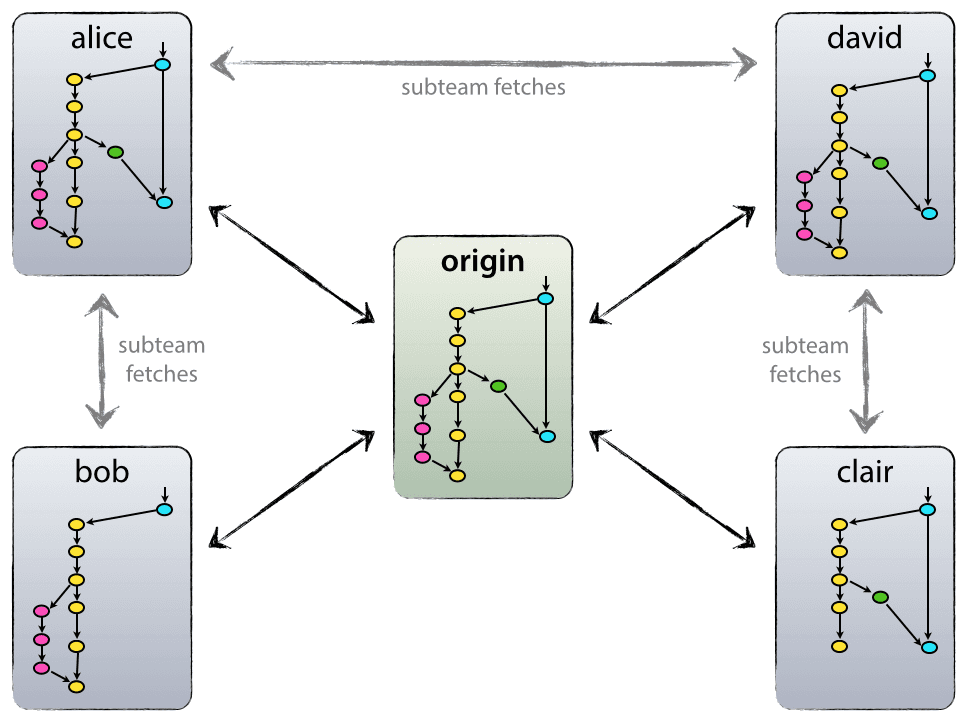
\includegraphics[height=0.8\textheight]{decentr}
    \end{figure}
\end{frame}

\begin{frame}
    \frametitle{Преимущества}
    \begin{itemize}
        \pause
        \item Локальные изменения
        \pause
        \item Отказоустойчивость
        \pause
        \item Довольный Линус
    \end{itemize}
\end{frame}

\begin{frame}
    \frametitle{Довольный Линус}
    \begin{figure}
        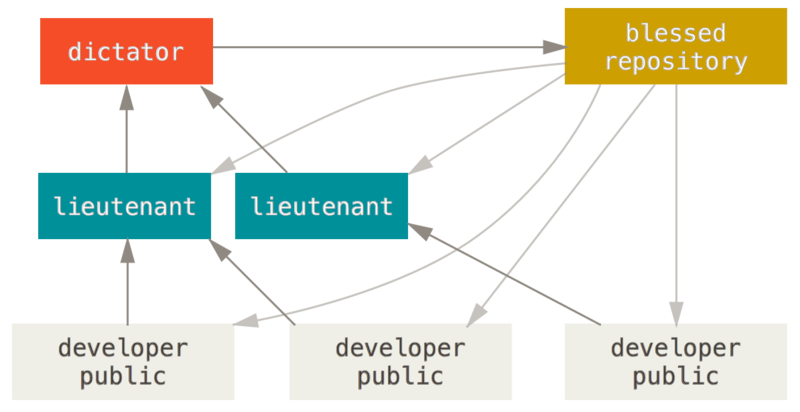
\includegraphics[width=\textwidth]{dictator}
    \end{figure}
\end{frame}

\section{Основные команды}

\begin{frame}[fragile]
    \begin{minted}{bash}
$ history | grep -P "^(\s|\d)*git" | awk '{ print $2, $3 }'
          | sort | uniq -c | sort -n -r
          | head -n 12
    304 git add
    300 git commit
    244 git checkout
    148 git push
    131 git diff
    110 git clone
     75 git rm
     69 git merge
     68 git remote
     62 git branch
     47 git reset
     45 git mv
    \end{minted}
\end{frame}

\begin{frame}[fragile]
    \begin{minted}{bash}
$ history | grep -P "^(\s|\d)*git" | awk '{ print $2, $3 }'
          | sort | uniq -c | sort -n -r
          | head -n 24 | tail -n 12
     25 git log
     17 git pull
     14 git check-ignore
     13 git ls-files
     10 git fetch
      9 git rebase
      6 git stash
      6 git cherry-pick
      5 git status
      5 git config
      4 git ls-tree
      3 git submodule
    \end{minted}
\end{frame}

\section{Советы}

\section{Продвинутые команды}

\section{GitHub}

\end{document}
